\documentclass{beamer}
\usetheme{Boadilla}
\setbeamertemplate{footline}[frame number]{}
\setbeamertemplate{navigation symbols}{}
\setbeamertemplate{footline}{}


\usefonttheme[onlymath]{serif}
\usepackage{mathtools, amssymb}
\usepackage{graphicx}
\graphicspath{{figures/}}

\newcommand{\diff}[2]{%
\dfrac{\mathrm{d^{#2}}#1}{\mathrm{d}t^{#2}}
}

\begin{document}

\begin{frame}{Switched Control of Inverted Pendulum}
\begin{columns}
\column{0.45\textwidth}
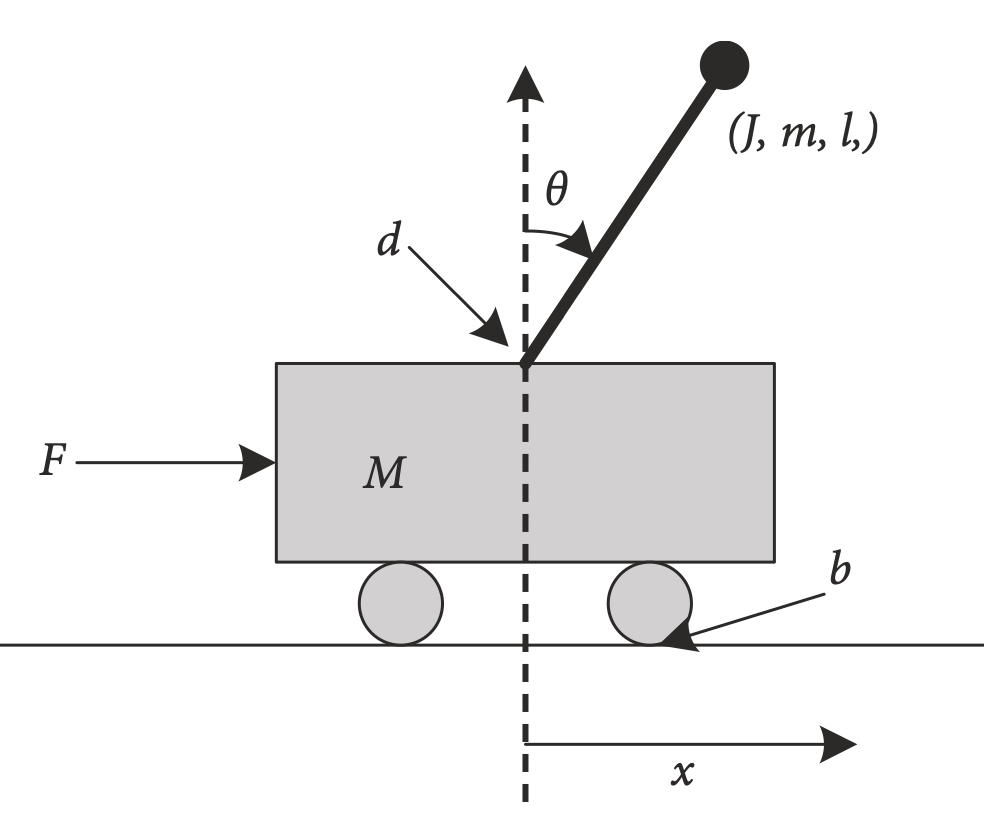
\includegraphics[width=\textwidth]{ip}  
\column{0.45\textwidth}
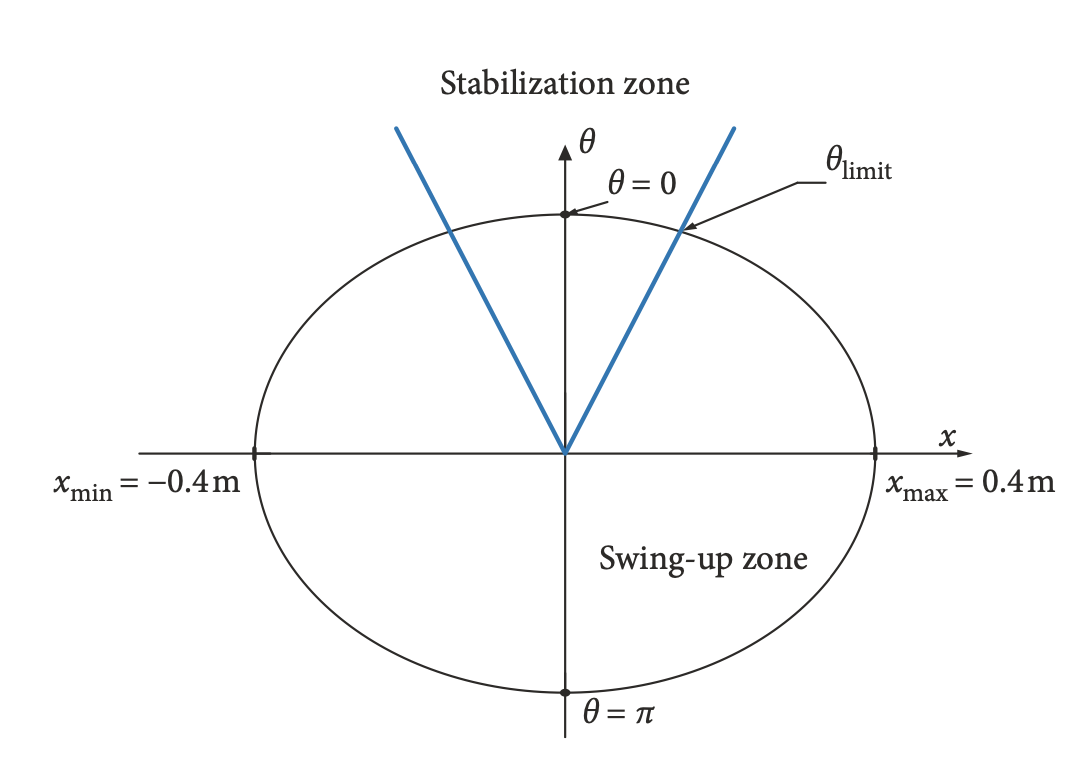
\includegraphics[width=\textwidth]{stz} 
\end{columns}
\begin{align*}
(m+M)\ddot{x} + b\dot{x} + ml\ddot{\theta}\cos(\theta) -ml\dot{\theta}^2\sin(\theta) &= F, \\
ml\ddot{x}\cos(\theta) + (J+ml^2)\ddot{\theta}-mfl\sin(\theta)+d\dot{\theta} &= 0. 
\end{align*} 
\end{frame}
   
\end{document}